% \begin{document}
\chapter{Probabilita' Condizionata}

\section{Definizione e motivazioni}

Supponiamo di sapere che un evento di un'esperimento aleatorio si e' avverato. Finora abbiamo visto solo casi in cui gli eventi non si influenzavano (\textit{indipendenti}), ma succede spesso nella realta' che se si sa che un certo evento e' avvenuto, allora questo ci da' informazioni aggiuntive che possono cambiare la probabilita' di altri eventi di cui ancora non sappiamo gli esiti.

Chiamiamo $ B $ l'evento che e' avvenuto e $ A $ un altro evento di cui vogliamo sapere la probabilita'. Prima di avere informazioni su $ B $, la probabilita' di $ A $ era semplicemente $ \mathbb{P}(A) $, ma ora ci poniamo la domanda: "se so che si e' verificato $ B $, come cambia $ \mathbb{P}(A) $?". Denotiamo questa nuova probabilita' con:
\[
  P(A|B)
\]
chiamata la \textit{probabilita' condizionata di  A  dato  B }.

\dfn{Probabilita' Condizionata}{
  Prendo due eventi $ A, B $ su uno spazio di probabilita' $ \left( \Omega, \mathbb{P} \right) $. Definisco \textit{probabilita' condizionata a B di A} la funzione:
  \begin{align*}
    \mathbb{P}(A|B): \powerset(\Omega) &\to [0,1]\\
    A &\mapsto \frac{\mathbb{P}(A \cap B)}{\mathbb{P}(B)}
  \end{align*}
}
E' possibile dimostrare che una certa funzione e' anch'essa una probabilita' (sempre discreta), verifichiamo gli assiomi (fissiamo $ B \subseteq \Omega $ con $ \mathbb{P}(B) > 0 $):
\begin{enumerate}
  \item $ \mathbb{P}(A|B) \in [0,1], \forall A \subseteq \Omega $
  \item $ \mathbb{P}(\Omega|B) = 1 $
  \item $ \sigma-\text{addittivita'} $: $ (A_i)_{i \in \mathbb{N}} $ disgiunti:
    \[
      \mathbb{P}(\bigcup_{i=1}^{\infty} A_i|B) = \sum_{i=1}^{\infty} \mathbb{P}(A_i|B)
    \]
\end{enumerate}
Lasciate al lettore in quanto davvero molto facili, quasi banali. Se non riesci a farle fai schifo.

Vediamo ora, con un esempio, come mai e' proprio questa la definizione utilizzata:
\ex{}{
  \begin{itemize}
  \item 
  Lancio del dado: $ \Omega = \{1,2,3,4,5,6\} $, $ \mathbb{P} $ probabilita' uniforme:

  $ \mathbb{P}(\{\omega\}) = \frac{1}{|\Omega|}, \forall \omega \in \Omega $, ovvero:
  \[
    \mathbb{P}(A) = \frac{\text{casi favorevoli in }A}{\text{casi possibili}}
  \]
  $ A = \text{"esce un numero maggiore di 3"} = \{3,4,5,6\} $ e $ B = \{\text{"esce un numero pari"}\} = \{2,4,6\} $, domanda: quanto vale $ \mathbb{P}(A|B) $?

  $ P(A) = \frac{4}{6} $ come abbiamo gia visto.

  Ora abbiamo un'informazione in piu': sappiamo che $ B $ si e' avverato. Questo significa che si restringe l'insieme di valori che possono essere usciti al lancio del dado. ATTENZIONE! cio' non vuol dire che cambia lo spazio campionario perche' l'esperimento e' lo stesso, ma cambiano i \textit{veri} casi favorevoli e i \textit{veri} casi possibili:
  \[
    P(A|B) = \frac{\text{"veri casi favorevoli di A"}}{\text{veri casi possibili}} = \frac{|A \cap B|}{|B|} = \frac{2}{3}
  \]
  \item
  Vediamo anche cosa accade quando la probabilita' non e' uniforme, come con un dado a 4 facce truccato: 

  $ \Omega = \{1,2,3,4\} $, $ \mathbb{P}(4)=\frac{1}{15}, \mathbb{P}(3)=\frac{2}{15}, \mathbb{P}(2)=\frac{4}{15}, \mathbb{P}(1)=\frac{8}{15} $

  $ A = \{3,4\}, B = \{2,4\} $
  \[
    \mathbb{P}(A|B) = \frac{\text{"probabilita' dei veri casi favorevoli di A"}}{\text{probabilita' dei veri casi possibili}} = \frac{\mathbb{P}(A \cap B)}{\mathbb{P}(B)}
  \]
  \end{itemize}

}

\nt{
  Se $ \mathbb{P} $ e' la probabilita' uniforme allora:
  \[
    \mathbb{P}(A|B) = \frac{\mathbb{P}(A \cap B)}{\mathbb{P}(B)} = \frac{\frac{|A \cap B|}{|\Omega|}}{\frac{|B|}{|\Omega|}} = \frac{|A \cap B|}{|B|}
  \]
}

\nt{
  B e' fissato nella definizione di propbabilita' condizionata, ovvero:
  \[
    \mathbb{P}(A|B) \neq \mathbb{P}(B|A)
  \]
  Quindi il ruolo di $ A $ e $ B $ e' completamente diverso
}

\nt{
  Se $ B = \Omega $, allora $ \mathbb{P}(A|B) = \mathbb{P}(A) $ dato che la conoscenza del fatto che si e' avverato $ \Omega $ e' ovvio e non ci cambia.

  Se $ A = \Omega $, allora $ \mathbb{P}(\Omega | B) = 1 $ (per proprieta', dato che e' sempre una probabilita')
}

\section{Regola della catena}

La probabilita' condizionata in genere e' nota e si usa per calcolare la probabilita' dell'intersezione:
  \[
    \mathbb{P}(A \cap B) = \mathbb{P}(A|B) \cdot \mathbb{P}(B)
  \]
Questa formula e' detta \textit{regola della catena} e vale in generale con $ n $ eventi:

\mprop{Regola della catena (generalizzata)}{
  $ (A_i)_{i = 1,...,n}, \mathbb{P}(A_1 \cap ... \cap A_{n-1}) > 0 $, allora:
  \[
    \mathbb{P}(A_1 \cap ... \cap A_n) = \mathbb{P}(A_1)\mathbb{P}(A_2|A_1)\mathbb{P}(A_3|A_1 \cap A_2) ... \mathbb{P}(A_n| A_1 \cap ... A_{n-1})
  \]
}
\nt{

  La condizione funziona grazie alla monotonia, dato che $ 0 < \mathbb{P}(A_1 \cap ... \cap A_{n-1}) \leq \mathbb{P}(A_1 \cap ... \cap A_j), 1 \leq j \leq n-1 $ quindi siamo certi che l'intersezione degli eventi che sono avvenuti e' maggiore di 0.
}
\pf{}{
  $ P(A_1) \frac{P(A_1 \cap A_2)}{P(A_1)}...\frac{P(A_1 \cap ... \cap A_n)}{P(A_1 \cap ... \cap A_{n-1})}= P(A_1 \cap ... \cap A_n) $
} 
TODO: migliora un po

\ex{}{
Un’urna contiene tre palline bianche, due palline nere e una pallina rossa.
Si eseguono tre estrazioni senza reimmissione.
Qual `e la probabilit`a di estrarre nell’ordine una bianca, una rossa e una nera?

  Sono interessato solo ad alcuni eventi, quindi non c'e' bisogno di descrivere l'intero esperimento aleatorio. Per prima cosa definisco l'evento:
  \[
  A = \text{"estrarre in ordine una bianca, una rossa e una nera"}
  \]
  Voglio trovare $ P(A) $. Notiamo che dobbiamo determinare tre sottoesperimenti in relazione (dato che non c'e' reimissione). Quindi dopo ogni sottoesperimento cambia la composizione dell'urna, e sappiamo come calcolare la probabilita' condizionata:
  \[
  B_i = \text{"estraggo una pallina bianca all' i-esimo turno"}
  \]
  \[
  R_i = \text{"estraggo una pallina rossa all' i-esimo turno"}
  \]
  \[
  N_i = \text{"estraggo una pallina nera all' i-esimo turno"}
  \]
  Esistono tre famiglie di eventi: $ (B_i)_{i = 1,...,k}, (R_i)_{i = 1,...,k}, (N_i)_{i = 1,...,k} $ dove $ i $ indica il turno al quale viene estratta la pallina. Quindi possiamo scrivere $ A $ come relazione fra sottoeventi:
  \[
  A = B_1 \cap R_2 N_3
  \]
  Quindi:
  \[
    P(A) = P(B_1 \cap R_2 \cap N_3) = P(B_1)P(R_2 | B_1)P(N_3 | B_1 \cap R_2)
  \]
  Solo ora possiamo passare ai valori numerici. Dato che gli esiti sono equiprobabili e lo spazio campionario e' finito, la probabilita' e' uniforme:
  \[
    P(B_1) = \frac{1}{2}, P(R_2) = \frac{1}{5}, P(N_3) = \frac{1}{2}
  \]
  \[
    P(A) = \frac{1}{20}
  \]
}

Per esperimenti formati da sottoesperimenti di cui conosco le probabilita' condizionate, e' possible rappresentare ogni evento come un nodo:
\[
\Omega = \text{primo nodo}
\]
e ogni probabilita' come un ramo che partiziona il nodo (tanti rami quanti gli insiemi della partizione) che rappresenta poi un altro evento (condizionato dalla seconda in poi).

\begin{center}
  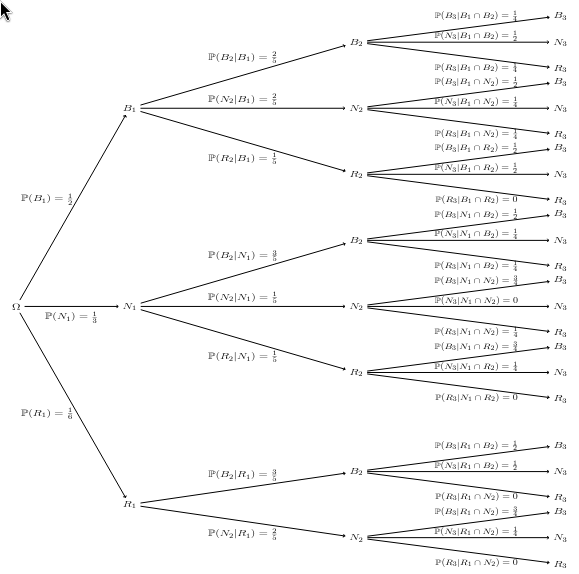
\includegraphics[width=0.5\textwidth]{img/2025-02-28-13-59-32.png}
\end{center}

La regola della catena la leggo sul diagramma ad albero:

percorso: $ \Omega \to B_1 \to R_2 \to N_3 $ ha probabilita' $ P(B_1 \cap R_2 \cap N_3) $ che si calcola facendo il prodotto delle probabilita' dei relativi rami che si usano nel percorso.

E' uno strumento utile per convincerci che stiamo usando le formule guiste, ma non le sostituisce e puo' diventare laborioso per problemi complessi.

\ex{}{
Ci sono due urne: la prima contiene due palline rosse e una bianca; la
seconda contiene tre palline rosse e due bianche. Si lancia una moneta: se esce testa si
estrae una pallina dalla prima urna, se esce croce si estrae una pallina dalla seconda urna.
Qual `e la probabilit`a che l’esito del lancio della moneta sia testa e la pallina estratta sia
bianca?

  2 sottoesperimenti:
  \begin{itemize}
  \item lancio della moneta
  \item estrazione da un'urna
  \end{itemize}

  Nota che i sottoesperimenti sono indipendenti dall'esito di altri esperimenti. Sono gli esiti, ovvero i risultati, che possono dipendere dagli esiti di altri esperimenti.

  \[
  A = \text{"esce testa ed estraggo una pallina bianca"}
  \]
  Devo esprimere A con eventi che 
  \[
  T = \text{"esce testa"}
  \]
  \[
  U = \text{estraggo una pallina bianca}
  \]
  Disegna lo zio pera di diagramma che non mi metto a fare, se @GiovanniPalma vuole puo' farlo
  \[
    A = T \cap U, \quad P(A) = P(T)P(U|T)
  \]
}

\section{Indipendenza di eventi}

E' possibile che sapere che un evento $ B $ e' avvenuto non altera la probabilita' di un altro evento $ A $. Possiamo esprimere questa relazione in modo matematico cosi':
\[
  \mathbb{P}(A|B) = \mathbb{P}(A)
\]
Utilizzando la definizione di probabilita' condizionata, possiamo usare un'identita' equivalente che useremo come definizione:
\dfn{Eventi indipendenti}{
  Due eventi $ A, B $ si dicono indipendenti se:
  \begin{equation}
    \mathbb{P}(A \cap B) = \mathbb{P}(A) \cdot \mathbb{P}(B)
  \end{equation}
  

  E viene denatato $A \dperp B$
}

Usiamo questa definizione dato che e' esplicitamente simmetrica, ovvero se A e indipendente a B allora vale anche il contrario:
\[
A \dperp B \iff B \dperp A
\]
ed e' definita (e banalmente vera) anche quando $ \mathbb{P}(A)=0 $ o $ \mathbb{P}(B)=0 $. In particolare si noti il seguente teorema:
\thm{Teorema della simmetria tra eventi indipendenti}{ \label{thm:simmetria_indipendenza}
  Sia $\mathbb{P}(B)>0$ allora:
  \[
    A \dperp B \iff \mathbb{P}(A|B) = \mathbb{P}(A)
  \]
  Dall'altro lato, sia $\mathbb{P}(A)>0$ allora:
  \[
    A \dperp B \iff \mathbb{P}(B|A) = \mathbb{P}(B)
  \]
}

\pf{Dimostrazione}{
  Verrà fornita solo la dimostrazione del primo punto, la seconda parte è analoga.

  Assumo $\mathbb{P}(B)>0$, si ha:
  \begin{itemize}
    \item $ A \dperp B \implies \mathbb{P}(A|B) = \mathbb{P}(A) $:
      \[
        \mathbb{P}(A|B) = \frac{\mathbb{P}(A \cap B)}{\mathbb{P}(B)} = \frac{\mathbb{P}(A) \cdot \mathbb{P}(B)}{\mathbb{P}(B)} = \mathbb{P}(A)
      \]
    \item $ \mathbb{P}(A|B) = \mathbb{P}(A) \implies A \dperp B $:
      \[
        \mathbb{P}(A \cap B) = \mathbb{P}(A|B) \cdot \mathbb{P}(B) = \mathbb{P}(A) \cdot \mathbb{P}(B)
      \]
  \end{itemize}
}

\nt{
  Si noti che se $\mathbb{P}(A)>0$ e $\mathbb{P}(B)>0$ allora, le tre uguaglianze seguenti sono equivalenti:
  \[
    \mathbb{P}(A\cap B) = \mathbb{P}(A) \cdot \mathbb{P}(B) \iff \mathbb{P}(A|B) = \mathbb{P}(A) \iff \mathbb{P}(B|A) = \mathbb{P}(B)
  \]
}

\nt{
  \begin{itemize}
  \item L'indipendenza e' diversa dalla disgiunzione:
  \[
  A \indip B \neq A \cap B = \emptyset
  \]
  infatti sono relazioni ortogonali:
  \[
    A \indip B \land A \cap B = \emptyset \iff \mathbb{P}(A)\mathbb{P}(B) = 0 \iff \mathbb{P}(A) = 0 \lor \mathbb{P}(B) = 0
  \]
  \item L'indipendenza e' diverso dall'essere sottoinsieme non-vuoto:
    \[
    A \indip B \neq A \subseteq B \lor B \subseteq A
    \]
    infatti:
    \[
      A \indip B \land A \subseteq B \iff \mathbb{P}(A)\mathbb{P}(B) = \mathbb{P}(A) \iff \mathbb{P}(B) = 1 
    \]
  \end{itemize}
  
  Quindi in generale due eventi sono indipendent quando la loro intersezione ha "le giuste proporzioni".
}

Adesso fornirò un altro teorema piuttosto importante:
\mprop{Sull'indipendenza di eventi complomentari}{
  Siano $A, B$ due eventi indipendenti, allora:
  \[
    A \dperp B \iff A^c  \dperp B,\, A \dperp B^c,\, A^c \dperp B^c
  \]
}
\pf{Dimostrazione}{
  Dimostro solo la prima parte, le altre sono analoghe.

  Assumo $A, B$ due eventi indipendenti, debbo dimostrare la seguente uguaglianza:
  \[
    \mathbb{P}(A^c \cap B) = \mathbb{P}(A^c) \cdot \mathbb{P}(B)
  \]

  Dato che 
  \[
    B = \Omega \cap B = (A \cup A^c) \cap B = (A \cap B) \cup (A^c \cap B)
  \]

  E dato che $ (A \cap B) $e$ (A^c \cap B)$ sono disgiunti, per \ref{item:finite_additivity} (\textit{additività finita}) si ha:
  \[
    \mathbb{P}(B) = \mathbb{P}(A \cap B) + \mathbb{P}(A^c \cap B)
  \]

  E dato che $ A \dperp B $ si ha:
  \[
    \mathbb{P}(B) = \mathbb{P}(A \cap B) + \mathbb{P}(A^c \cap B) = \mathbb{P}(A \cap B) = \mathbb{P}(A) \cdot \mathbb{P}(B) + \mathbb{P}(A^c \cap B)
  \]
  Quindi:
  \[
    \mathbb{P}(A^c \cap B) = \mathbb{P}(B) - \mathbb{P}(A \cap B) = \mathbb{P}(B) - \mathbb{P}(A) \cdot \mathbb{P}(B) = \mathbb{P}(B) \cdot (1 - \mathbb{P}(A)) = \mathbb{P}(A^c) \cdot \mathbb{P}(B)
  \]
}

\subsection{Generalizzazione su n eventi}

Come nel caso con solo due eventi, $ n > 2 $ eventi si dicono indipendenti quando, sapendo che qualsiasi numero degli altri eventi si e' avverato, la probabilita' dell'evento non cambia. Questo deve valere per tutti gli $ n $ eventi, ovvero:
\[
  \mathbb{P}\left(A_i \middle\vert \bigcup_{j=1, j\neq i}^{n} A_j\right) = P(A_i) \quad \forall i = 1,...,n
\]
Si puo' dimostrare, usando la definizione di probabilita' condizionata, che questa identita' equivale a dire:
\dfn{Eventi indipendenti (per n eventi)}{
  Sia $ (A_i)_{i \in I} $ una famiglia di eventi in uno spazio di probabilita'. Si dice che questi eventi sono indipendenti quando \textbf{per ogni sottoinsieme} finito $ J \subseteq I.\ |J| > 2 $:
  \[
    \mathbb{P} \left( \bigcap_{j \in J} A_j \right) = \prod_{j \in J} \mathbb{P}(A_j)
  \]
}

\subsection{Esercizi}

\ex{Calcolo di eventi indipendenti con probabilita condizionata}{

\textbf{TESTO:}

    Si lancia un dado a 6 facce

    \( A = \) "Esce un numero \( > 4 \)" \\
    \( B = \) "Esce un numero pari"

    Determinare \( P(A) \) e \( P(A|B) \)

\textbf{DETTAGLIO SVOLGIMENTO:}

    \begin{align*}
        \Omega &= \{1, 2, 3, 4, 5, 6\} \\
        A &= \{ 5, 6\} \\
        B &= \{2, 4, 6\} \\
        P(A) &= \frac{3}{6} = \frac{1}{3} \\
        P(A|B) &= \frac{P(A \cap B)}{P(B)} = \frac{\frac{1}{6}}{\frac{3}{6}} = \frac{1}{3}
    \end{align*}

    Dato che \( P(A) = P(A|B) \), per il teorema \ref{thm:simmetria_indipendenza} si ha che \( A \dperp B \)
}

Ecco un altro eserzio:
\ex{}{
  \textbf{TESTO}

Lanciamo una moneta e un dado a 4 facce.

Determinare uno spazio di prob. che descriva l'esperimento aleatorio

\textbf{SOLUZIONE}

$\Omega = \left\{ (T,1), (T,2), (T,3), (T,4), (C,1), (C,2), (C,3), (C,4) \right\}$

$P(T,1) = \frac{1}{8} = P(C,4) = \frac{1}{8}$

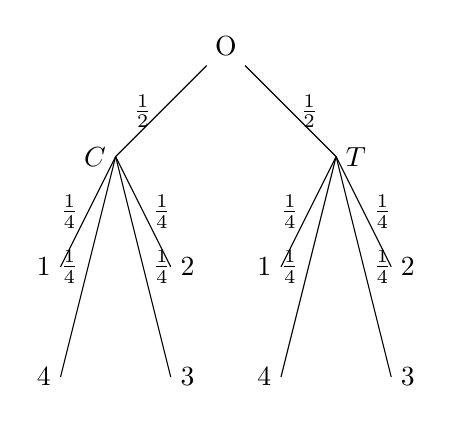
\begin{tikzpicture}[scale=0.7]
    \node (root) at (0,0) {O};
    \draw (root) -- (-2,-2) node[left] {$C$} node[midway,left] {$\frac{1}{2}$};
    \draw (root) -- (2,-2) node[right] {$T$} node[midway,right] {$\frac{1}{2}$};
    
    \draw (-2,-2) -- (-3,-4) node[left] {$1$} node[midway,left] {$\frac{1}{4}$};
    \draw (-2,-2) -- (-1,-4) node[right] {$2$} node[midway,right] {$\frac{1}{4}$};
    \draw (-2,-2) -- (-1,-6) node[right] {$3$} node[midway,right] {$\frac{1}{4}$};
    \draw (-2,-2) -- (-3,-6) node[left] {$4$} node[midway,left] {$\frac{1}{4}$};
    
    \draw (2,-2) -- (1,-4) node[left] {$1$} node[midway,left] {$\frac{1}{4}$};
    \draw (2,-2) -- (3,-4) node[right] {$2$} node[midway,right] {$\frac{1}{4}$};
    \draw (2,-2) -- (3,-6) node[right] {$3$} node[midway,right] {$\frac{1}{4}$};
    \draw (2,-2) -- (1,-6) node[left] {$4$} node[midway,left] {$\frac{1}{4}$};
\end{tikzpicture}

  \[
  \begin{aligned}
  & T = \text{"esito del lancio moneta e testa"} \\
  & C = \text{"esito del lancio moneta è croce"} \\
  & D_i = \text{"è uscito il numero } i \text{"} \\
  & P(C) = \frac{1}{2}, \quad P(T) = \frac{1}{2} \\
  & P(D_i | C) = \frac{1}{4} \\
  & P(D_i | T) = \frac{1}{4} \\
  & A = \text{"è uscito testa e il numero } i \text{"} \\
  & P(A) = P(T) \cdot P(D_i | T) = \frac{1}{2} \cdot \frac{1}{4} = \frac{1}{8} \\
  & \text{Analogamente per } C \cap D_i
  \end{aligned}
  \]
}



% \end{document}
